The next experiment we ran was to measure the amount of time it takes to run a procedure of 0-7 integer parameters and 1 returned integer.

Thus we implement experiment functions of this form: 
\begin{verbatim}
unsigned function(unsigned x_1, unsigned x_2){
  return 0;
}

static inline unsigned long execute(){
  return function(1, 2);
}
\end{verbatim}

To execute the procedure we have to load the arguments to registers, add the return pointer to the stack and then move the instruction pointer twice(there/back).
We suspect there are about 10 instructions per procedure call with 2 additional per parameter.  Most of these instructions deal with memory and thus will take a couple cycles each.  Thus we suspect about 20 cycles + 6 cycles per parameter.


\begin{figure}[h]
\centering
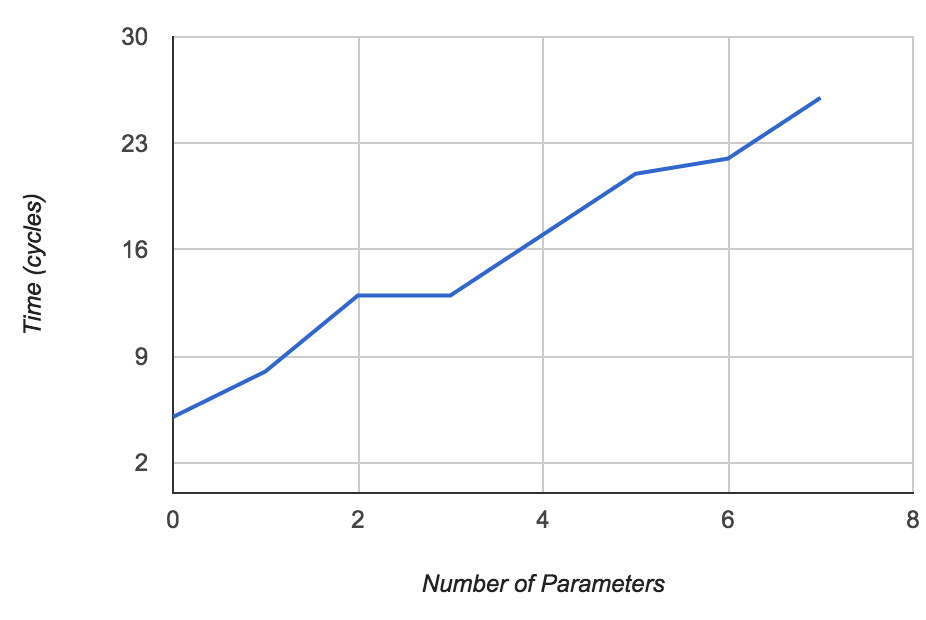
\includegraphics[scale=.5]{experiments/exp_1_2_fig.png}
\caption{Mean execution time vs number of parameters.  Overhead time included for comparison.  The standard deviation for all experiments was under 1 ns}
\end{figure}

There was a ~15 cycle overhead for procedure calls over the do nothing overhead.  Thus we were pretty close in our expected additional overhead for procedure calls.  There is also a strong linear relationship between number of procedure arguments and the time taken.  By performing a linear regression we get 4.2 ns additional cost per argument or about 3  additional cycles per parameter.